6. $\cfrac{(x^2-1)(2x^2+5x-7)}{3-x}\leqslant0\Leftrightarrow\cfrac{(x-1)^2(x+1)\cdot 2\left(x+\cfrac{7}{2}\right)}{3-x}\leqslant0.$ Применив метод интервалов, найдём ответ:
\begin{figure}[ht!]
\center{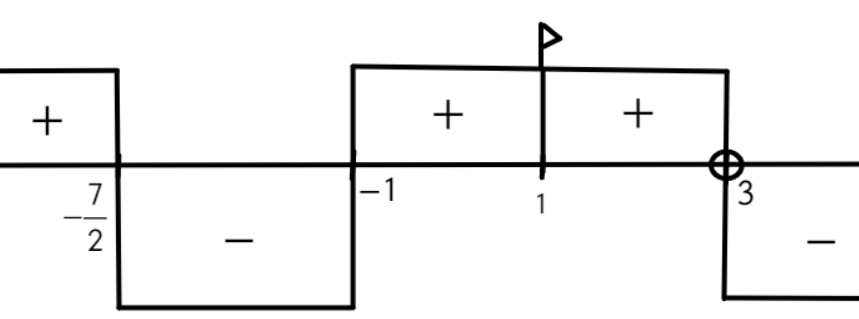
\includegraphics[scale=0.35]{int6.png}}
\end{figure}
$x\in\left[-\cfrac{7}{2};-1\right]\cup\{1\}\cup(3;+\infty).$\\
